\section{Piecewise models as mixture models}
\label{sect:mix}
%%%%%%%%%%%%%%%%%%%%%%%%%%%%%%%%%%%%%%
%We begin by considering Gibbs sampling on 
In this section we overcome the exponential complexity of standard Gibbs
sampling by transforming piecewise models to (augmented) mixture models and performing
linear time Gibbs sampling in this augmented model.  
We motivate the algorithm by formula~\ref{e:expanded}:
It represents a Bayesian inference model in which likelihood functions are piecewise.
% Good point, but no space. -Scott
%
%\footnote{Clearly, prior distributions can be piecewise as well but since exponential blow up in the posterior structure is due to the amount of data, our focus is on likelihood functions.}
For readability, case statements are numbered and without loss of
generality, we assume the number of partitions in each
likelihood function is $M$:
\begin{align}
\label{e:expanded}
pr(\boldsymbol\theta | \, d_1, \ldots, d_n) \, 
\propto \,
pr(\boldsymbol\theta) \otimes
{\footnotesize
\begin{cases}
\boxed{k_1 = 1.} &{\phi^{1}_{1}(\boldsymbol\theta)  : f^{1}_{1}(\boldsymbol\theta)}\\
\vdots
\\
\boxed{k_1 = M.} &\phi^{1}_{M}(\boldsymbol\theta)  \!:\! f^{1}_{M}(\boldsymbol\theta)
\end{cases}
}%end font size
\!\!
\otimes
\cdots
\otimes
{\footnotesize
\begin{cases}
\boxed{k_n = 1.} &\phi^{n}_{1}(\boldsymbol\theta)  : f^{n}_{1}(\boldsymbol\theta)\\
\vdots
\\
\boxed{k_n = M.} &\phi^{n}_{M}(\boldsymbol\theta)  \!: f^{n}_{M}(\boldsymbol\theta)
\end{cases}
}%end font size
%\\= {\footnotesize
%\begin{cases}
%\phi_{1, 1}(\boldsymbol\theta) \wedge \ldots \wedge \phi_{n, 1}(\boldsymbol\theta) : f_{n, 1}(\boldsymbol\theta) \ldots f_{n, 1}(\boldsymbol\theta)\\
%\vdots
%\\
%\phi_{1, M}(\boldsymbol\theta) \! \wedge\! \ldots \!\wedge\! \phi_{n, M}(\boldsymbol\theta) \!:\! f_{n, 1}(\boldsymbol\theta) \ldots f_{n, M}(\boldsymbol\theta)
%\end{cases}
%}%end font size
\end{align} 
In the above, $k_i$ is the partition-counter of the $i$-th likelihood function. 
$\phi^i_{j}$ is its $j$-th constraint and
 $f^i_{j}$ is its associated sub-function. 
%Remembering that $\phi^i_{1}$ to $\phi^i_{M}$ are mutually exhaustive and jointly exhaustive, 

We observe each $k_i$ can be seen as a random variable. 
It deterministically takes the value of the partition whose associated constraint holds (given $\boldsymbol\theta$) and its possible outcomes are in $\textsc{Val}(k_i) = \{1, \ldots, M\}$. 
Note that by the way we defined piecewise functions, given any $\boldsymbol\theta$, 
on each piecewise function exactly one constraint holds. Therefore, 
$\sum_{k_i = 1}^M pr(k_i \,|\, \boldsymbol\theta) = 1$.
Intuitively, it can be assumed that $k_i$ are underlying variables determining which partition of each likelihood function is `chosen'.  
If we can show that: 
\begin{equation}
\label{e:aaaax}
pr(d | \, \boldsymbol\theta) = \sum_{k = 1}^M pr(k | \, \boldsymbol\theta) pr(d | \, k, \boldsymbol\theta)
\end{equation}
we can claim that a piecewise likelihood functions can be seen 
as mixture models in which sub-functions $f^i_j$ are \emph{mixture components} and 
 $k_i$ provide binary \emph{mixture weights}. And from there is follows that:
%$$pr(d_i | \boldsymbol\theta) = \sum_{k_1}pr(k_1 | \, \boldsymbol\theta) pr(d_1 | \, k_1, \boldsymbol\theta)$$
%and
%\[pr(k_i = k \,|\, \theta) := {\footnotesize
%\begin{cases}
%\phi^i_k(\boldsymbol\theta)  &: 1\\
%\neg \phi^i_k(\boldsymbol\theta) &: 0
%\end{cases}
%}%end font size
%\]
%Provided with this definition, by Proposition~\ref{pro:discrete}, equation~(\ref{e:expanded}) can be restated as:
\begin{align*}
pr(\boldsymbol\theta | \, d_1, \ldots, d_n) 
&\propto
pr(\boldsymbol\theta) \otimes
\sum_{k_1}pr(k_1 | \, \boldsymbol\theta) pr(d_1 | \, k_1, \boldsymbol\theta) \otimes
\cdots \otimes
\sum_{k_n}pr(k_n | \, \boldsymbol\theta) pr(d_n | \, k_n, \boldsymbol\theta)
\\
&\propto
\sum_{k_1} \ldots \sum_{k_n} p(\boldsymbol\theta, d_1, \ldots, d_n, k_1, \ldots, k_n) 
\end{align*}
This means that Bayesian networks in Figures~\ref{fig:naive} and \ref{fig:naive.mix} are equivalent.
Therefore, instead of taking samples from \ref{fig:naive}, 
they can be taken from the \emph{augmented model} \ref{fig:naive.mix} 
A key observation, however, is that 
unlike the conditional distributions $pr(\theta_i | \, \boldsymbol\theta_{-i})$, 
in $pr(\theta_i | \boldsymbol\theta_{-i}, k_1, \ldots, k_n)$ 
the number of partitions remains fixed rather than growing $O(M^n)$.
%As an instance, for $n=2$,   $k_1 = M$ and $k_2 = 1$:

The reason is that if  $k_1, \ldots, k_n$ are given, for an $i$-th likelihood, a single sub-function $f^i_{k_i}$ is `chosen' and:
$pr(\theta_i | \boldsymbol\theta_{-i}, k_1, \ldots, k_n) = 
pr(\boldsymbol\theta | \boldsymbol\theta_{-i})\prod_{k_i} f^i_{k_i}(\theta_i | \boldsymbol\theta_{-i})$.
Assuming that sub-functions are not piecewise themselves, 
the amount  of partitions in $pr(\theta_i | \boldsymbol\theta_{-i},  k_1, \ldots, k_n)$ is bound by the amount of partitions in the prior.

What is remained is to show that equation~\ref{e:aaaax} is valid:
%\[
%p(x_i |\, \bvec{x}_{i-1}, \bvec{k}) = 
 % f_{1, 2}(\bvec{x}) \ldots f_{n, 2}(\bvec{x})
%\]  
\begin{comment}
\begin{equation}
\label{e:dodo}
pr\left(
{\footnotesize
\begin{cases}
{\phi^{1}_{1}(\boldsymbol\theta)  : f^{1}_{1}(\boldsymbol\theta)}\\
\vdots
\\
\boxed{\phi^{1}_{M}(\boldsymbol\theta)  : f^{1}_{M}(\boldsymbol\theta)}
\end{cases}
}
\otimes 
{\footnotesize
\begin{cases}
\boxed{\phi^{2}_{1}(\boldsymbol\theta)  : f^{2}_{1}(\boldsymbol\theta)}\\
\vdots
\\
\phi^{2}_{M}(\boldsymbol\theta)  :  f^{2}_{M}(\boldsymbol\theta)
\end{cases}
}
, k_1 = M, k_2 = 1\right)
= f^{1}_{M}(\boldsymbol\theta)  f^{2}_{1}(\boldsymbol\theta)
%end font size
\end{equation}


\section{Piecewise models as mixture models}
\label{sect:mix}

Consider a piecewise likelihood function in equation~(\ref{e:piecewise.likelihood22}). 
A simple but key observation is that since the constraints, $\phi_j$, exhaustively partition the space of $\boldsymbol \theta$,
we can define an \emph{auxiliary} (or \emph{augmented}) random variable $k$ with $M$ possible outcomes, $\text{Val} (k) := \{1, \, \ldots, \, M\}$,
such that 
$pr(k = i |\, \boldsymbol\theta) = 1$ if and only if $\phi_i (\boldsymbol\theta) = \top$. %\footnote{Note that $\sum_{k_i} pr (k_i | \, \boldsymbol \theta) = 1$.}%end footnote. 
As the following shows,
a piecewise model can be reinterpreted as a \emph{mixture model} 
which is the result of marginalizing over the \emph{intermediate} random variables $k$.
This means that graphical models depicted in Figures~\ref{fig:naive} and \ref{fig:naive.mix} are equivalent.
\end{comment}
%%%%%%%%%%%%%%%%%%%%%%%%%
\begin{figure}
\centering
\begin{subfigure}{.40\textwidth}
\centering
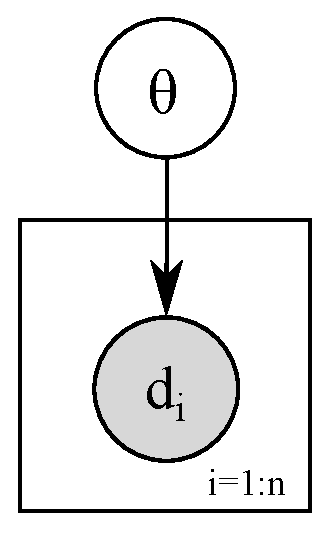
\includegraphics[width=.28\textwidth]{pic/naive.pdf}
\caption{}
\label{fig:naive}
\end{subfigure}
\begin{subfigure}{.40\textwidth}
\centering
  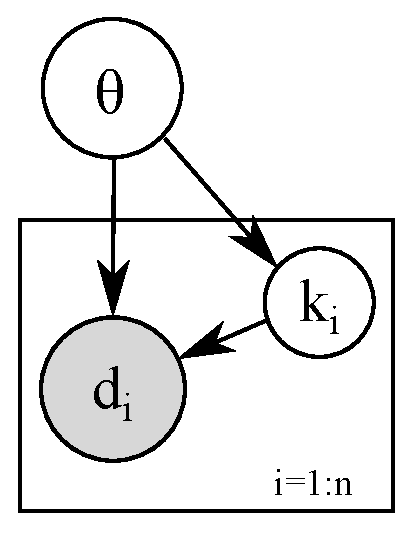
\includegraphics[width=.35\textwidth]{pic/naive-mix2.pdf}
\caption{}
\label{fig:naive.mix}
\end{subfigure}
\caption{\footnotesize 
(a) A Bayesian inference model with parameter (vector) $\boldsymbol\theta$ and data points $d_1$ to $d_n$.
(b) A mixture model with parameter (vector) $\boldsymbol\theta$ and data points $d_1$ to $d_n$ 
}
\end{figure}
%%%%%%%%%%%%%%%%%%%%%%%

%----------------------------------------***
\begin{proposition}
\label{pro:discrete}
Piecewise likelihood function $pr(d | \, \boldsymbol\theta)$ 
defined by (\ref{e:piecewise.likelihood22}) is equivalent to 
$\sum_{k = 1}^M pr(k | \, \boldsymbol\theta) pr(d | \, k, \boldsymbol\theta)$
where:

\noindent\begin{minipage}{.5\linewidth}
\begin{equation}
\label{e:piecewise.likelihood22}
pr(d | \, \boldsymbol\theta) :=
{\footnotesize
\begin{cases}
\phi^d_1(\boldsymbol\theta)  &: f^d_1(\boldsymbol\theta)\\
\vdots\\
\phi^d_M(\boldsymbol\theta)  &: f^d_M(\boldsymbol\theta)
\end{cases}
}%end font size 
\end{equation} 
\end{minipage}%
\begin{minipage}{.5\linewidth}
\begin{equation}
\label{e:2rel22}
pr(k |\, \boldsymbol\theta) := 
{\footnotesize
\begin{cases}
\phi_k(\boldsymbol\theta)  &: 1\\
\neg \phi_k(\boldsymbol\theta) &: 0
\end{cases}
}%end font size
\end{equation}
\begin{equation}
\label{e:2rel222}
  pr(d | \, k, \boldsymbol\theta) := f_k(\boldsymbol\theta, d)
\end{equation}
\end{minipage}

%
\end{proposition}
\begin{proof}
Since constraints $\phi_k$ are mutually exclusive and jointly exhaustive: 
$$\sum_{k= 1}^N pr(k | \, \boldsymbol\theta) = 
\sum_{k=1}^N
{\footnotesize
\begin{cases}
\phi_k(\boldsymbol\theta)   &: 1\\
\neg \phi_k(\boldsymbol\theta)  &: 0
\end{cases}
}%end font size
\, =1
$$
Therefore $pr(k | \, \boldsymbol\theta)$ is a proper probability function. 
On the other hand, by marginalizing $k$, (\ref{e:2rel22}) and (\ref{e:2rel222}) trivially lead to (\ref{e:piecewise.likelihood22}):
\begin{align*}
\sum_{k} pr(k | \, \boldsymbol\theta)pr(d | \, k, \boldsymbol\theta) 
&= 
\sum_{k=1}^N  
{\footnotesize
\begin{cases}
\phi_k(\boldsymbol\theta)  &: 1\\
\neg \phi_k(\boldsymbol\theta) &: 0
\end{cases}
}%end font size
\, \cdot \, f_k(\boldsymbol \theta, d)
&&\text{by (\ref{e:2rel22}), (\ref{e:2rel222})}
\\
&=
\sum_{k=1}^N 
{\footnotesize
\begin{cases}
		\phi_k(\boldsymbol\theta)  &: f_k(\boldsymbol\theta, d)\\
\neg 	\phi_k(\boldsymbol\theta)  &: 0
\end{cases}
}%end font size
= {\footnotesize
\begin{cases}
\phi_1(\boldsymbol\theta)  &: f_1(\boldsymbol\theta, d)\\
\vdots\\
\phi_n(\boldsymbol\theta)  &: f_N(\boldsymbol\theta, d)
\end{cases}
}%end font size
= pr(d | \, \boldsymbol\theta) 
&&\text{by (\ref{e:piecewise.likelihood22})}
\end{align*}
in which the third equality holds since constraints $\phi_k$ are mutually exclusive. 
\end{proof}
%Proposition~\ref{pro:discrete} shows that a piecewise model can be augmented to an equivalent model  via augmenting it with auxiliary random variables. The difference is that the order of complexity of Gibbs sampling on the latter model is significantly lower.However, two subtle problems are remained that will be addressed in the next subsections. %as the next subsection shows, it causes a \emph{deterministic dependencies problem} that should be addressed first.
 
\subsection{Deterministic dependencies and blocked sampling}
\label{sect:deterministic}
%%%%%%%%%%%%%%%%%%%%%%%%%
\begin{figure}
  \centering
  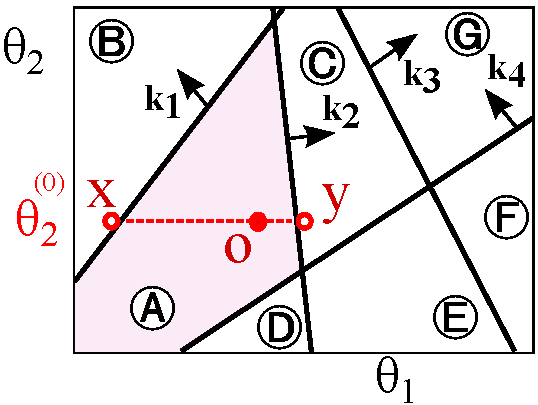
\includegraphics[width=0.35\textwidth]{pic/colxx.pdf}
\caption{\footnotesize
A piecewise joint distribution of $(\theta_1, \theta_2)$ partitioned by bi-valued linear constraints.
% with associated auxiliary variables $k_i$.
In the side specified by each arrow its associated auxiliary variable $k_i$ is 1 otherwise 2.
A Gibbs sampler started from an initial point $O = (\theta_1^{(0)}, \theta_2^{(0)})$, is trapped in an initial partition (A) 
where $k_1 = k_2 = k_3 = 1$ and $k_4 = 2$. 
}
\label{fig:simple.example}
\end{figure}
%%%%%%%%%%%%%%%%%%%%%%%
\paradot{Deterministic dependencies} It is known that in the presence of determinism Gibbs sampling gives poor results \cite{Poon:06}.
In our setting, deterministic dependencies arise from Definition~(\ref{e:2rel22}), were the value of $k$ is  decided by $\boldsymbol{\theta}$.
This problem is illustrated in Figure~\ref{fig:simple.example} by a simple example:
A Gibbs sampler started from an initial point $O=(\theta_1^{(0)}, \theta_2^{(0)})$, 
is trapped in the initial partition (A). 
The reason is that conditioned on the initial value of the auxiliary variables, the partition is deterministically decided as being (A), and conditioned on any point in (A), the auxiliary variables are decided to keep their initial values. %I.e.\ only on line segment $xy$, $pr(\theta_1 | \theta_2^{(0)}, k_1^{(0)}, \ldots, k_4^{(0)}) >0$, etc.

%To illustrate the problem that emerges by Gibbs sampling on the mixture model defined by Proposition~\ref{pro:discrete}, consider the simple piecewise model depicted in Fig.~\ref{fig:simple.example} on a 2D parameter space $\boldsymbol\theta = (\theta_1, \theta_2)$ with a 2-piece prior, two observed points with a 2-piece and a 3-piece corresponding likelihood models. We augment the model by introducing auxiliary random variables $\bvec{k} = \{k_1, k_2\}$ such that $\textsc{Val}(k_1) = \{1,2,3\}$ and $\textsc{Val}(k_2) = \{1,2\}$ indicating (the constrain of) which partition in each likelihood function holds. Suppose Gibbs sampling is executed on the augmented model, starting from an initial point $(\theta_1^{(0)}, \theta_2^{(0)}, k_1^{(0)} = 2, k_2^{(0)} = 1)$ (shown in Fig~\ref{fig:blocking}a as a filled red circle). Firstly, $\theta$ is conditionally sampled: $\theta_1^{(1)} \sim pr(\theta_1 | \, \theta_2^{(0)}, k_1^{(0)}, k_2^{(0)}) $ In Fig~\ref{fig:blocking}a, the interval on which this conditional distribution is non-zero is depicted with a red dashed line segment. Clearly $\theta_1^{(1)}$ will be located inside partition (A) or (B) where $k_1 = 2$ and $k_2 = 1$ (i.e.\ second constraint of the first likelihood and the first constraint of the second likelihood function hold). In the second step, $\theta_2$ is sampled (see Fig.~\ref{fig:blocking}b): $\theta_2^{(1)} \sim pr(\theta_2 | \, \theta_1^{(1)}, k_1^{(0)}, k_2^{(0)})$ which again lies in either (A) or (B). In the next step  $k_1^{(1)} \sim pr(k_1 | \, \theta_1^{(1)}, \theta_2^{(1)}, k_2^{(0)})$ would deterministically take its former value $k_1^{(0)}$ since it is decided by $\boldsymbol\theta^{(1)}$. Similarly, $k_2^{(1)} = k_2^{(0)}$. By following this process, it can clearly be seen that all generated particle(s) will remain in the union of partitions (A) and (B).  This example reveals that Gibbs sampling on an augmented model is trapped in an initial set of partitions that specify the initial value of auxiliary variables). A way round this problem is provided in the next subsection.  
%%%%%%%%%%%%%%%%%%%%%%%%%%%%%%
%\subsection{Blocked Gibbs sampling on mixture models}
%\label{sect:collapsed}
\paradot{Blocked Gibbs}
We avoid deterministic dependencies by Blocked sampling:
at each step of Gibbs sampling, a parameter variable $\theta_i$ is jointly sampled with  
(at least) one  
auxiliary variable $k_j$ 
conditioned on the remaining variables:
$
(\theta_i, k_j) \sim pr(\theta_i, k_j | \, \boldsymbol \theta_{-i}, \bvec{k}_{-j})  
$.
%(\emph{blocked Gibbs sampling}).
Since 
$pr(\theta_i, k_j | \, \boldsymbol \theta_{-i}, \bvec{k}_{-j}) = 
pr(\theta_i | \, \boldsymbol \theta_{-i}, \bvec{k}_{-j}).pr(k_j | \, \boldsymbol\theta)$,  
this is done in 2 steps:
\begin{enumerate}
\item 
$k_j$ is marginalized over and $\theta_i$ is sampled (\emph{collapsed Gibbs sampling}):
$$
\theta_i \sim \sum_{k_j} 
pr(k_j | \, \boldsymbol \theta_{-i}, \bvec{k}_{-j}) 
pr(\theta_i | \, k_j, \boldsymbol \theta_{-i}, \bvec{k}_{-j})  
$$
\item
$k_j$ is determined from $\boldsymbol \theta$:
$k_j \leftarrow i \in \textsc{Val}(k_j)$ s.t.\ $\phi_i^j(\boldsymbol \theta) \equiv \top$
where $\phi_i^j$ is the $i$-th constraint of $j$-th likelihood function.
\end{enumerate}

For instance, if in Figure~\ref{fig:simple.example} for Gibbs sampling from $\theta_2$, either $k_1$ or $k_2$ in collapsed,
then the next sample will be in the union of partition (A) with either (B) or (C). 

%This trick is illustrated in Fig.~(\ref{fig:blocking}c) where $(\theta_1, k_2)$ are sampled jointly, followed by joint sampling of $(\theta_2, k_1)$ in (in Fig.~\ref{fig:blocking}d). 
%Using this method, (at least for some combinations of auxiliary and parameter variables) deterministic dependencies does not occur. This prevents being trapped in a single subset of partitions.
\paradot{Targeted selection of collapsed auxiliary variables}
We provide of a mechanism for finding auxiliary variables $k_j$ that, with a high  probability, are not determined by the other auxiliary variables, $\bvec{k}_{-j}$ when jointly sampled with a parameter variable $\theta_i$. 
We observe that the set of partitions satisfying the current valuation of $\bvec{k}$
often differs with its adjacent partitions in a single auxiliary variable.
Since such a variable is not determined by other variables, it can be used in the blocked sampling.
However, in case some likelihood functions share a same constraint, some adjacent partitions would differ in multiple auxiliary variables.
In such cases, more than one auxiliary variable should be used in blocked sampling.

Finding such auxiliary variables has a simple geometric interpretation. Therefore, instead of trying to formalize the solution, we explain it by a simple example depicted in Figure~(\ref{fig:simple.example}): 

Consider finding a proper $k_j$ 
for blocked sampling $pr(\theta_1, k_j | \, \theta_2^{(0)}, \bvec{k}_{-j})$. 
It suffices to extend the line segment $pr(\theta_1 | \, \theta_2^{(0)}, \bvec{k})>0$ in two sides to reach the point $x$ or $y$. In this way, the neighboring partition e.g.\ (B) and (C) and consequently their corresponding $\bvec{k}$ valuations are detected. 
Finally, the auxiliary variables that differ between (A) and (B) or differ between (A) and (C)) are found ($k_1$ and $k_2$, in the Figure~(\ref{fig:simple.example})). 
%Clearly by block sampling these variables with $\theta_1$, deterministic dependency problem is avoided.
%By comparing the auxiliary variables that differs between (C) and the union of (A) \& (B) which is $k_2$. This is exactly how, blocked sampling is carried out in Fig.~\ref{fig:blocking}. 

\begin{comment}
More generally, 
to avoids deterministic dependencies in sampling 
$\theta_i \sim pr(\theta_i | \, \boldsymbol\theta, \bvec{k})$,   
the auxiliary variable(s) $\bvec{k}_j$ that are block sampled with $\theta_i$ , are selected as follows:

1.  A point $\widehat{\boldsymbol{\theta}}$ in a neighboring partition is found:
$\widehat{\boldsymbol \theta}_{-i} \leftarrow {\boldsymbol \theta}_{-i}$ and
with probability 0.5, $\widehat{\theta}_i \leftarrow \theta_i^L$ otherwise $\widehat{\theta_i} \leftarrow \theta_i^U$ where 
% Two points that are at the opposite ends of the line segment $pr(\theta_i = \theta | \, \boldsymbol{\theta}_{-i}, \bvec{k})>0$ but are not included in it are taken:
\begin{align*}
\theta_i^L := \inf   \{ \theta_i \,|\,\, p(\theta_i | \, \boldsymbol{\theta}_{-i}, \bvec{k})>0 \} - \epsilon
\qquad
\theta_i^U := \sup \{ \theta_i \,|\,\, p(\theta_i | \, \boldsymbol{\theta}_{-i}, \bvec{k})>0 \} + \epsilon
\end{align*}
and $\epsilon>0$ is a small number.

2. Let  
$\widehat{\bvec{k}} = (\widehat{k}_1, \ldots, \widehat{k}_n)$ 
be the valuation of auxiliary variables in the found neighboring region.
%\begin{align*}
%\widehat{\bvec{k}} \leftarrow (\widehat{k}_1, \ldots, \widehat{k}_n) \text{ s.t. }
%\widehat{k}_j = i\in \textsc{Val}(k_j) \text{ where } \phi_i^j(\boldsymbol \theta) \equiv \top
%\end{align*}
%where $\phi^i_l$ is the $l$-th constraint of the likelihood function associated with the $i$-th observation. 
The set $\bvec{k}^b$ of auxiliary variables that should be used in blocked sampling with $\theta_i$ consists of auxiliary variables that differ between the current partition and its neighbor: 
$\bvec{k}^b = \{k_i | k_i \neq \widehat{k_i} \}$ for $j = 1, \ldots n$.
%\begin{align*}
%\bvec{k}^b = \{\widehat{k} \in \widehat{\bvec{k}} | \, k_x \neq \hat{k}_x\}
%\end{align*} 
\end{comment}
